\documentclass{elsarticle}
\usepackage{amssymb}
\usepackage{hyperref}
\usepackage{graphics}
\journal{Expert System with Applicaitons}

\newtheorem{definition}{Definition}
\begin{document}

\begin{frontmatter}


\title{Knowledge Acquisition Method from Domain Text Based on Theme Logic Model and Artificial Neural Network \tnoteref{t1,t2}}
\tnotetext[t1]{This document is a collaborative effort.}
\tnotetext[t2]{The second title footnote.}

% use optional labels to link authors explicitly to addresses:
% \author[label1,label2]{}
% \address[label1]{}
% \address[label2]{}

\author[buaa]{Jun Wang\corref{cor1}}
\ead{king.wang@buaa.edu.cn}
\author[buaa]{Yunpeng Wu\corref{cor2}}
\ead{yunpeng.wu@sem.buaa.edu.cn}
\author[buaa]{Xuening Liu\corref{cor2}}
\ead{xx@gmail.com}


\cortext[cor1]{Corresponding author}
\cortext[cor2]{Principal corresponding author}
\fntext[fn1]{This is the specimen author footnote.}
\fntext[fn2]{Another author footnote, but a little more longer.}



\address[buaa]{School of Economics \& Management, Beihang University, Beijing 100083,
P.R. China }


\begin{abstract}
% Text of abstract
In order to acquire knowledge from domain text such as failure analysis text of aviation product, a framework is proposed to enhance the efficiency and accuracy of knowledge acquisition. In this framework, sentence templates are defined to extract the meta-knowledge and RDF is used to manage the extracted knowledge.  After the preprocessing steps, we propose a new model theme logic model (TLM) to present all the themes in a text and the logic relations between different themes. In this model, the text of each theme can be represented as an attribute-value vector based on domain ontology, and the logic relation is the domain knowledge to be acquired. Then the theme logic model will be transformed to the training set of the artificial neural network to acquire the failure analysis knowledge. After training the knowledge acquired will be extracted by SD method from the artificial neural network and represented by rules. At last, a prototype is developed to acquire knowledge from failure analysis reports of aviation product. Empirical results show that the framework can acquire knowledge from domain text efficiently.
\end{abstract}

\begin{keyword}
% keywords here, in the form: keyword \sep keyword

% PACS codes here, in the form: \PACS code \sep code

% MSC codes here, in the form: \MSC code \sep code
% or \MSC[2008] code \sep code (2000 is the default)
Knowledge Acquisition; Domain Text; Theme Logic Model; Artificial Neural Network; Failure Analysis Report


\end{keyword}

\end{frontmatter}

\section{Introduction}
\label{sec:introduction}

Over the past decades, massive volumes of data have been collected in
corporations, of which more than eighty percent is stored in
text \cite{Mitchell2003}. But unfortunately, the explosive growth of
information has often resulted in frustrating situations when
corporations are not able to organize the information well and
understand the knowledge it contains. Knowledge management is
implemented by enterprise and organization to manage their knowledge
more effectively. According to Turban and Aronson, knowledge
management includes sorting useful knowledge from information, storing
knowledge in good order, and finding knowledge in an existing
knowledge base \cite{turban2001dss}. Knowledge acquisition from text
(KAT) is to extract knowledge contained in texts and is an important
way of knowledge acquisition. The text collection in a specific domain
can be called domain text. The label ‘domain text’, in this term,
means that although written in natural language, the content of the
text is closely related to a specific domain. These texts have two
main characteristics: on the one hand, the set of terms used to
describe their contents, and on the other, a well-defined structure to
organize these contents comprehensibly and improve readability for the
user \cite{Campos2004}. The text follows a certain controllable syntax
which can be easily summarized and formulated. Thus the domain text
referred in this paper is semi-structured. 

The domain knowledge is valuable but often buried in domain text within a range of sources such as failure analysis reports of aviation product, government files, records of meetings and experimental reports, to name a few. The domain text collection can be mined to learn about a subfield. Through automated approaches, knowledge correlated to a specific domain can be extracted and integrated from these disparate text sources. The knowledge acquired is valuable for a variety of applications including decision support, quality assurance and knowledge retrieval.

There have been many research efforts devoted to automatic knowledge
acquisition from text \cite{salton1975vsm,361220,215383,Tai2002,130346} . The early
knowledge acquisition systems operate on the principal of indexing the
texts in the collection using Boolean model. The model is over
simplify and cannot rank the relevant texts together with automatic
indexing, so Salton proposed Vector Space Model (VSM) in 1975 \cite{salton1975vsm,361220}. In this model, text is represented by vectors in a multidimensional space. According to the literature, VSM is the most popular and effective indexing approach \cite{215383}. To improve the performance of VSM, a number of enhanced methods have been proposed. These approaches include methods based on dimensionality reduction and methods using feedback information from the user \cite{Tai2002}. The former centers on reducing the high-dimensional vector space into a low-dimensional one, among them the Latent Semantic Indexing (LSI) using Single Valued Decomposition is probably used most widely \cite{130346}. The latter uses feedback information from a user to increase the effectiveness.

In this research, we focus on developing an effective methodology of knowledge acquisition from domain text such as failure analysis reports of aviation product based on a new text indexing model, theme logic model. Salton described text themes as a main text decomposition strategy \cite{234834}. The text theme is represented by semantically homogeneous text pieces where all components treat a common subject area. The theme logic model employs two sets to represent a text: a set of themes in the text and a set of relations among the themes. The text of each theme can be represented as an attribute-value vector based on domain ontology, so the set of themes is a set of vectors of all the themes in the text. In addition, there are meaningful logic relation existing between different themes, and for a domain the logic relation is the domain knowledge to be acquired. Artificial neural network belong to the family of learning-by-example paradigm in which problem-solving knowledge is automatically generated according to actual examples \cite{Huang2002,Kim2004}. The theme logic model will be transformed to the training set of the artificial neural network to acquire the failure analysis knowledge. Then the knowledge acquired will be extracted by SD method from the artificial neural network and represented by rules \cite{130346,Sestito1991}. Furthermore, a prototype system is implemented and tested for scenario demonstration. Empirical results show that the framework can acquire knowledge from domain text efficiently.

The paper is organized as follows. In Section 2 we review some related work about knowledge acquisition from text and failure analysis. We then propose the framework of knowledge acquisition in detail in Section 3. The structure analysis of domain text is presented in Section 4. In Section 5 we describe how to construct the theme logic model of domain text based on the domain ontology. And then in Section 6, we use BP neural network to acquire the knowledge based on the theme logic model. At last, in Section 7 we show some experimental results and discussion and in Section 8 we give some conclusions. 

\section{Related Work
}
\label{sec:related-work}

\subsection{Knowledge Acquisition from Text
}
\label{sec:knowl-acqu-from}

Knowledge acquisition from text is one of the most fruitful research
areas in artificial intelligence. Text-based knowledge acquisition
methods and tools can help to manage the wealth of information and
discover facts, relationships and implications in domain texts
\cite{Hahn2000,Gunn1999}. 

Gunn et al discusses existing knowledge acquisition techniques based
on manual learning, machine learning and logic programming [21]. The
manual learning methodology relies on knowledge engineers to acquire
and formalize knowledge from experts or free texts. However, any
natural language is extremely difficult for computer systems to
understand, the machine learning and inductive logic programming
methodologies both require at least some manual processing of the
large quantity of source information \cite{matwin:tac,Richardson1997}. Training set and background knowledge must be built to aid and the interaction of knowledge engineers is necessary. And the result of an inductive system can never be guaranteed to be accurate because identification of relevant features and selection of representative examples are important to this approach. None of the aforementioned KA techniques seem adequate for acquiring knowledge from domain text, for the reasons given. 
Most knowledge acquisition systems operate on the principal of
indexing the texts in the collection. The most popular indexing
approach is based on the vector space model [5][6]. According to the
literature, VSM is the most effective methodology [7]. In this model,
text is represented by vectors in an n-dimensional space, where n is
the number of distinct terms. There are three-step strategy where
terms are first extracted from the document text, then the weights of
the indexed terms are derived to improve the document retrieval
accuracy, and then the documents are ranked with respect to a
similarity measure \cite{Raghavan1986}. To improve the performance of
VSM, a number of enhanced methods have been proposed. The reduction of
the dimensionality of the model is one way to solve these
problems. The LSI model is accomplished by mapping a high-dimensional
space into a low-dimensional space by using SVD. Wenlei Mao and Wesley
W. Chu discuss three types of schemes, the stem-based, concept-based
and phrase-based schemes, and show the retrieval effectiveness of the
phrased-based VSM is significantly higher than that of the current
gold-standard—the term-based VSM \cite{Mao2007}. Chih-Ping Wei et
al. propose an LSI-based multilingual document clustering technique
that employs LSI analysis to a parallel corpus and constructs a
multilingual semantic space, which reduces the dimensions and thereby
improves both clustering effectiveness and efficiency \cite{Wei2008}.

\subsection{Failure Analysis
}
\label{sec:failure-analysis-}

Failure, as defined by the International Electro-technical Commission (IEC), is ‘the termination of the ability of an item to perform a required function’. Whenever a failure occurs, the failed component and the failure situation must be examined to determine the cause. This investigation process is called failure analysis \cite{Liao1999}. Robert suggests that there should be a systematic way of performing failure analysis and the investigation and analysis process will follow a logical series of stages \cite{roberts1980stm}. An opinion regarding the failure mechanism will be formed and a final conclusion will be reached by the domain experts. Finally, a failure analysis will be written to note the entire process of failure analysis. The failure analysis report is an important source of engineering knowledge, which contains substantial and essential failure knowledge and conveys some inherent phenomena or regularities about the processes generating failure. Acquiring knowledge from failure analysis report will lead to design, material selection or fabrication modifications and important economies \cite{Castro2004}. 
Traditionally, the failure analysis process is carried out by vast
numbers of human experts. However, as the volume of failure analysis
report is growing at explosive rates, this process become extremely
ineffective and inefficient. The availability and use of accurate
knowledge acquisition from this large volume is
required. Computer-assisted knowledge acquisition is necessary to
support quality decision-making and help to overcome human cognitive
constraints.  Numerous studies have been conducted to develop
computer-assisted systems and various approaches have been taken such
as fault tree analysis [30], expert systems \cite{Kim2004}, neural
network \cite{Zakarian1999}, neuro-fuzzy system [33], etc. Mayer described an expert system for electric utility power plant personnel to identify a basic failure mechanism that can produce the type of boiler tube failure under investigation []34. T. Warren Liao developed an integrated database and expert system for indentifying the failure mechanism of mechanical components \cite{liao1999ida}. Relatively fewer attempts have been made to develop computerized failure analysis systems whose knowledge is acquired from domain text such as failure analysis report.


\section{A Framework for Knowledge Acquisition from Domain Text
}
\label{sec:fram-knowl-acqu}

The aim of this framework is to acquire knowledge from semi-structure
domain texts. The knowledge acquisition is processed through several
modules including structure analysis, theme logic model construction
and artificial neural network, as shown in Figure 1. The structure
analysis transforms the failure analysis report into unique RDF by
defining sentence templates. The theme logic model represents all the
texts based on domain ontology using two sets: a set of all themes in
a text and a set of the relations among the themes. The ontology is
frame-oriented and a set of classes, relations, attributes and
values. The artificial neural network processes a train set
transformed from the theme logic model based on the domain ontology,
and the acquired knowledge will be extracted by SD method and
represented by rules. At last, the acquired knowledge rules will be
stored into a knowledge base.
\begin{figure}[htp]
  \centering
  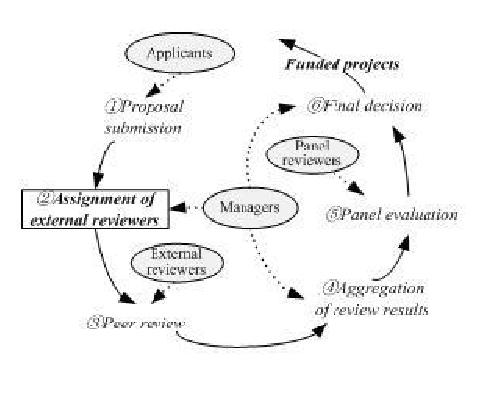
\includegraphics{esa/1.eps}

  \caption{The Framework for Knowledge Acquisition from Domain Text}
  \label{fig:1}
\end{figure}

\section{Structure Analysis of Domain Text 
}
\label{sec:struct-analys-doma}

There are tremendous domain texts in an enterprise, so the first step
is to transform them to a unique format. The main purpose of the
structure analysis and meta-knowledge acquisition is to analyze the
structure of the domain text and use meta-knowledge to help to manage
them. As the base of OWL, RDF offers a generic framework and plays an
important role in the construction of semantic web \cite{lassila1999rdf}. Thus we
choose RDF and the output of the structure analysis is a set of RDF
documents, as is shown in Figure2. 
\begin{figure}[htp]
  \centering
  \includegraphics{esa/2.eps}

  \caption{Transform failure analysis report into RDF}
  \label{fig:2}
\end{figure}
Although written in natural language, the content of the domain text is closely related to a specific domain and follows a certain controllable syntax which can be easily summarized and formulated. Thus the domain text referred in this paper is semi-structured. The main steps of transform are:
Step1 Analyze domain texts set T-Set, and define a grammar G used for defining the information extraction rule;
Step2 Define the information extraction rules set R;
Step3 Build a validator to test whether R conforms to all the domain texts;
Step4 If there are texts violate R, return to Step 3;
Step5 Write a parser to analyze the texts and find text blocks
matching rule in R, transform T-Set to R-Set.  

The purpose of structure analysis of domain text is to find the
modeling ways based on the structural characteristics of the domain
for the further access to acquire knowledge and effectively improve
the accuracy and effectiveness of other follow-up
text-processing. Salton described two main text decomposition
strategies, including a chronological decomposition into text segments
and semantic decomposition into text themes \cite{234834}. The text segment is
a contiguous piece of text units that is linked internally, but
largely disconnected from the adjacent text. The text theme is
represented by semantically homogeneous text pieces where all
components treat a common subject area.

As to the failure analysis report, it is usually in a certain format
in accordance with the requirements for writing, and can be called a
semi-structured text. The well-defined structure is used to organize
the content comprehensibly and improve readability for the user. Thus
the text segment and the text theme are easily to be found and
described. The text themes focus on the structure that contains the
text of the ideological content and logical way of expression.

\begin{itshape}
  The text segments of failure analysis report= (title, author,
  abstract, chapter, section, paragraph, sentence). 

The text themes of failure analysis report= (title, author, abstract, phenomenon of the failure component, reasons and inference for the failure, judgment of the failure mode).

\end{itshape}

Salton used vector space model to represent the structure of the
text. In this model, text is represented by vectors in an
n-dimensional space, where n is the number of distinct
terms. According to the literature, VSM is the most effective and
popular indexing approach. There are three-step strategies where terms
are first extracted from the document text, then the weights of the
indexed terms are derived to improve the document retrieval accuracy,
finally the documents are ranked with respect to a similarity measure.
v
In addition, different types of texts have different forms of
organization, and paragraph is a basic organizational
hierarchy. Different paragraphs constitute a hierarchy to express the
common theme in an orderly manner. The division of text theme is based
on the common subjects expressed by several paragraphs. And logic
relations often exist between different themes of a text. As to
failure analysis report, the three themes  phenomenon of the failure component’, ‘reasons and inference of failure’, ‘judgment of failure mode’ consist three themes and there are meaningful logic relations among them. Failure analysis report is a form record of the entire failure analysis process, in which the domain experts use the failure analysis techniques to do experiment, observe and analyze the failure phenomena to determine the reasons for failure and make the necessary preventive measures based on their own knowledge in a particular field \cite{roberts1980stm}. Therefore, the logic relation between the themes ‘phenomenon of the failure component’ and ‘judgment of failure mode’ is the essential logic mapping from failure phenomenon to failure mode, which is the very failure knowledge to be acquired. Therefore, we build a new theme logic model to express the logic relation between different themes.



\begin{definition}
  The theme logic model of a text with n different themes is :
\[ d = (T = \{T_1,T_2,\ldots,T_n\}, R = \{R_{ij} = R(T_i,T_j) \, | \, T_i,T_j \in
T,1\le i,j \le n \}) \]
where $T$ represents a set of themes in the text, $R$ represents a set of logic relation between two themes, $R_{ij}$ represents the logic relation between themes $T_i$ and $T_j$. 

\end{definition}

\section{Theme Logic Model of Dom
}
\label{sec:theme-logic-model}

In order to acquire the domain knowledge of failure analysis, we
choose two themes ‘Phenomenon of the failure component’ (represented
by P) and ‘judgment of failure Mode’ (represented by M) to construct
the theme logic model of failure analysis report as $d = (T = \{P,M\},
R = \{R_{PM}\})$.

$R_{PM}$ represents the logic relation between theme $P$ and $M$ and
is the domain knowledge to be acquired. In failure analysis, the
domain experts use their tacit knowledge to relate various phenomenons
with a specific failure mode, but the tacit knowledge in their mind is
not easily to be expressed and transformed to explicit knowledge even
by the domain experts themselves, and that is the reason why the
knowledge acquisition becomes the bottleneck in knowledge
engineering. We will construct the theme logic model of the domain
texts and transform them into the training set of artificial neural
network to acquire the knowledge. More precisely, the text in each
theme will be represented to an attribute-value vector based on the
domain ontology. 

The failure analysis techniques use by domain experts are relatively fixed, such as trace analysis, crack analysis and fracture analysis. Each analysis techniques observe phenomenon of failure component from different angles. And the phenomenon observed and the attributes of each phenomenon can be clearly described by domain ontology. In addition, the language and sentence structure to express and describe the failure phenomenon are usually relatively fixed. Therefore, the text of each theme can be presented by an attribute-value vector in an n-dimensional space based on lightweight domain ontology of failure analysis, which is frame-oriented and a set of classes, relations, attributes and values \cite{747902}.

\begin{definition}
  The attribute-value vector of theme $T_i$ in text is defined as:
\[AVV_i = \{<a_1,v_1>,<a_2,v_2> \ldots,<a_n,v_n>\} \]
\end{definition}
$a_i$ represent the attributes in theme $T_i$, and vi represents the value of attribute $a_i$ , $n$ is the number of distinct attributes in domain ontology.

\begin{definition}
  A lightweight domain ontology ($O$) models a specific domain, and is
  made up of a set of Concepts ($C$), Attributes ($A$), Attribute
  Value ($V$) and Relations between the Concepts ($R$):$O = \{C,A,V,R\}$


\end{definition}

Concepts (or classes) are the abstract nodes or collections of objects. Attribute provides extra features used to identify and describe the concept. Each attribute has at least a name and a value, and is used to store information that is specific to the object it is attached to. In addition, the value of an attribute can be a complex data type, such as a numerical interval or a set. Relation is used to indicate a similarity between two concepts within ontology. The four elements are shown in Figure 3.
\begin{figure}[htb]
  \centering
  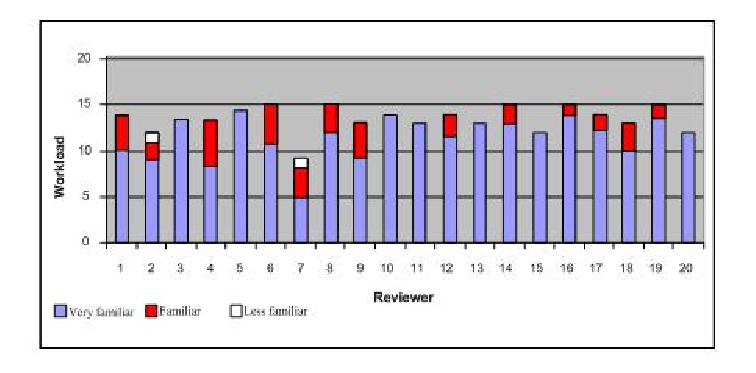
\includegraphics{esa/3.eps}
  \caption{Elements in Lightweight Domain Ontology}
\end{figure}
There are three steps to construct attribute-value vector.
Step1 Pretreatment
For the text of each theme in RDF documents to be processed, all the standing alone punctuation marks are removed first and the text will be divided into sections by full stop and comma.
Step2 Construct lightweight domain ontology 
The lightweight domain ontology comprises two sub-ontology: failure analysis technique ontology and failure mode ontology. Ontology construction is a large and tedious task. But here we only need lightweight domain ontology to express all the concepts, relations, attributes and values. Thus it is much easier to construct it. What’s more, a synonym base will be also included to store all the words having the same or nearly the same meaning as the attribute and attribute value in a language.
Step3 Extract attribute-value vector based on lightweight domain ontology
We do word segmentation and use string matching to identify and collect the attributes and values based on the lightweight domain ontology. The similarity of attribute (or attribute value) S1 of string S2 is defined as follows.
\begin{definition}
  Similarity of Attribute (or Value) S1 of String
  S2 \[similarity(S_1,S_2) = \frac{V(S_1) \cap V(S_2)}{V(S_1)} \]

\end{definition}

$V(S_1)$ represents the number of single words in $S_1$, and $V(S_1)
\cap V(S_2)$ represents the common single words in $S_1$ and $S_2$.

The algorithm to construct attribute-value vector is as follows. ‘a’ and ‘b’ are two indicators of similarity.

\begin{verbatim}
Input: 
A theme in RDF
Lightweight domain ontology 
String[] GetSynonymy (String) //a function to get the synonym of a word

Output:
attribute-value vector of a theme

Algorithm:
Each sentence in the theme is divided into sub sections by full stop and comma to form a vector of sub sentence vector={C1,C2,…,Ci,…,Cn} 

For each Ci, i=1,2,..n 
For each ai of Ontolgoy 
aSyn=GetSynonymy(ai)
    Foreach s of aSyn
	  Search s in Ci
       IF similarity>a THEN
		 For each vi,j of ai
  			vSyn=GetSynonymy(ai)
    			 For each c of vSyn
				Search c in Ci
        			IF similarity> THEN
				Add < ti, vi,j> to attribute-value vector
			    ELSE Next c
  ELSE Next s

\end{verbatim}

\section{Knowledge Acquisition Based on Theme Logic Model and Artificial Neural Network}
\label{sec:knowl-acqu-based}

Artificial neural network belongs to the family of learning-by-example paradigm in which problem-solving knowledge is automatically generated according to actual examples \cite{hassoun1995fan}. As there is a very complicated nonlinear relation between the phenomena of failure and the failure mode, it is difficult to establish a suitable model in practice. Artificial neural network with its adaptive, self-learning and non-linear system of powerful analytical capacity provides a new solution for failure analysis. The main steps include:
Step1 Design the architecture of artificial neural network.
Step2 Transform the theme logic model into the training set of the neural network, train and test the neural network. 
Step3 Extract knowledge from neural network and represent the
knowledge with rules.

\subsection{Artificial Neural Network Design}
\label{sec:artif-neur-netw}

The ANN can be classified into several categories based on supervised
and un-supervised learning methods and feed-forward and feedback
recall architectures. The back-propagation network algorithm (BPNN) is
a multi-layered network first proposed by Rumelhart
\cite{rumelhart1986lir}. The algorithm is also called a supervised
learning method that can be used to solve non-linear problems. The
learning stage of BPNN involves a forward pass and a backward pass. An
advantage of BPNN is that it does not need to change the network
structure or activation functions of nodes and only adjusts the
weights between nodes in the network [40]. BPNN is one of the most
frequently utilized neural network techniques for classification and
prediction \cite{graupe2007pan}. In this research, we also use the
BPNN architecture in a supervised learning method to acquire knowledge
from domain text. The neural network is concerned with acquiring
failure knowledge from a set of data consisting of the theme logic
model. 

BPNN architecture comprises an input layers, an output layer and hidden layers. The BPNN parameters include a number of hidden layers, a number of hidden neurons, an activation function, learning rate, momentum, etc. All of these have significant impact on the performance of BPNN.
\begin{itemize}
\item The input neurons are used to represent the phenomena of failure component, which is according to the attribute value of failure analysis technique ontology. For each attribute-value vector.
\item The output neurons are used to reflect the failure mode of failure component. There are different hierarchies of failure mode. We can assign the output neurons to reflect a specific hierarchy of failure mode and the knowledge mapping the phenomena to this hierarchy of failure mode will be acquired. 
\item One hidden layer is sufficient for computing arbitrary decision
  boundaries for the output in most cases [42]. It is import to
  mention that there is no standard formula for calculating the number
  of nodes in the hidden layer [43]\cite{turban:oaj}. Maren, Harston
  and Pap demonstrated that the bound of neurons in the hidden layer
  was between $2N_i+1$ and $N_o(N_i +1)$, where $N_i$ is the number of
  input nodes and No is the number of output nodes
  \cite{maren1990hnc}. The number of hidden nodes are selected through
  experiment between $2N_i+1$ and $N_o(N_i +1)$. 
\item The activation function is mathematical formula that determines the output of a processing neuron. Logistic activation functions are employer in the hidden layer and linear activation is utilized in the output layer.  
\item As to the learning rate and momentum, most ANN software package provides default values for both parameters that typically work well. The learning rate determines the speed at which the weight change and the momentum constant prevent sudden changes in attaining the results.  


\end{itemize}

\subsection{Transform the Theme Logic Model to Training Set}
\label{sec:transf-theme-logic}

Every training sample is represented by theme logic model, and then every theme in the mode will be represented by an attribute-value vector as the training data of the BPNN. The P theme will be transformed to attribute-value vector based on the failure analysis technique ontology, and be used as the input vector of the BPNN. While the M theme will be transformed to attribute-value vector based on the failure mode ontology, and be used as the output vector of the BPNN. Each attribute value in ontology will be included in the input vector or output vector. For an attribute-value vector of a theme to be transformed, if the attribute value exist in it, we assign the attribute value to 1 in the input vector else to 0. 

After transformation, we get a set of n-dimensional input vector. We put the entire input vectors transformed from m sample texts together to form the input matrix. 
\[\begin{array}{cccccc}
    V_1&V_2&\cdots&V_j&\cdots&V_n
\end{array}
\newline
\left[  
  \begin{array}{cccccc}
    V_1&V_2&\cdots&V_j&\cdots&V_n
  \end{array} \right]
\]



\bibliographystyle{elsarticle-num}
\bibliography{../../bibtex/elsevier,../../bibtex/emerald,../../bibtex/chinese,../../bibtex/jstor,../../bibtex/citeseer,../../bibtex/acm,../../bibtex/wiley,../../bibtex/book,../../bibtex/thesis,../../bibtex/ebsco,../../bibtex/old,../../bibtex/ieee.bib,../../bibtex/springer,../../bibtex/internet}

\end{document}
